\documentclass[a4paper,oneside,12pt]{extreport}
\usepackage[T2A,T1]{fontenc}
\usepackage[utf8]{inputenc}
\usepackage[english,russian]{babel}

\usepackage[left=30mm, right=15mm, top=20mm, bottom=20mm]{geometry}

\usepackage{microtype}
\sloppy

\usepackage{setspace}
\onehalfspacing

\usepackage{indentfirst}
\setlength{\parindent}{1.25cm}

\usepackage{titlesec}
\titleformat{\chapter}{\LARGE\bfseries}{\thechapter}{20pt}{\LARGE\bfseries}
\titleformat{\section}{\Large\bfseries}{\thesection}{20pt}{\Large\bfseries}

\titlespacing*{\chapter}{0pt}{0pt}{20pt}


\usepackage{wrapfig}
% \usepackage{float}

% \makeatletter
% \renewcommand{\fnum@figure}{Рисунок \thefigure}
% \makeatother


\usepackage{pgfplots}
\pgfplotsset{compat=newest}

\usepackage{listings}
\lstset{
	basicstyle=\footnotesize\ttfamily,
	keywordstyle=\color{blue},
	stringstyle=\color{red},
	commentstyle=\color{gray},
	numbers=left,
	numberstyle=\tiny,
	numbersep=5pt,
	frame=false,
	breaklines=true,
	breakatwhitespace=true,
}

\newcommand{\code}[1]{\texttt{#1}}

\usepackage{amsmath}
\usepackage{amssymb}

\usepackage{tikz}
\usetikzlibrary{arrows}
\usetikzlibrary{shapes}

\usepackage{booktabs}
\usepackage{array}
\usepackage{adjustbox}

\usepackage{enumerate}

\usepackage[unicode]{hyperref}
\hypersetup{hidelinks}

\makeatletter
\def\vhrulefill#1{\leavevmode\leaders\hrule\@height#1\hfill \kern\z@}
\makeatother


\usepackage{csvsimple}

\usepackage{caption}
\usepackage[justification=centering]{caption}
% \captionsetup{justification=centering}


\def\lab{6}
\def\topic{Расстояние Левенштейна и Дамерау-Левенштейна}
\def\topic{Алгоритмы умножения матриц}
\def\topic{Алгоритмы сортировки}
\def\topic{Параллельные вычисления}
\def\topic{Многопоточная реализация конвейера}
\def\topic{Муравьиный алгоритм и полный перебор}
% \def\topic{Поиск в словаре}


\begin{document}

\begin{titlepage}
	\centering
	\large
	
	\begin{wrapfigure}[7]{l}{0.14\linewidth}
		\vspace{5mm}
		\hspace{-5.8mm}
		
\includegraphics[width=0.93\linewidth]{../../report/common/bmstu-logo}
	\end{wrapfigure}
	{\singlespacing \footnotesize \bfseries Министерство науки и высшего образования Российской Федерации\\Федеральное государственное бюджетное образовательное учреждение\\высшего образования\\<<Московский государственный технический университет\\имени Н.~Э.~Баумана\\ (национальный исследовательский университет)>>\\(МГТУ им. Н.~Э.~Баумана)\\}

	\vspace{-2.2mm}
	\vhrulefill{0.9mm}\\
	\vspace{-7.5mm}
	\vhrulefill{0.2mm}\\
	\vspace{2mm}
	
	{\doublespacing \normalsize \raggedright ФАКУЛЬТЕТ \hspace{25mm} «Информатика и системы управления»\\
	КАФЕДРА \hspace{5mm} «Программное обеспечение ЭВМ и информационные технологии»\\}

	\vspace{30mm}
	
	\textbf{ОТЧЕТ}\\
	По контрольной работе № 1\\
	По курсу: <<Анализ алгоритмов>>\\
	Тема: <<\topic>>\\

	\vspace{60mm}

	\hspace{70mm} Студент:      \hfill Ле Ни Куанг\\
	\hspace{70mm} Группа:       \hfill ИУ7и-56Б\\
	\hspace{70mm} Преподаватель:\hfill Волкова Л. Л.\\
								\hfill Строганов Ю. В.\\
	% {\raggedright \hspace{70mm} Оценка: \hfill \hrulefill\\}

	\vfill
	
	Москва\\
	\the\year
\end{titlepage}

\setcounter{page}{2}
\tableofcontents

\chapter*{Введение}
\addcontentsline{toc}{chapter}{Введение}


Параллельные вычисления - способ организации компьютерных вычислений,
при котором программы разрабатываются как набор взаимодействующих вычислительных процессов, работающих параллельно (одновременно).
\\


\textbf{Целью работы:} изучение параллельных вычисления
с использованием алгоритма Винограда.
В данной лабораторной работе реализовать
последовательный и параллельный алгоритм Винограда.
\\

\textbf{Задачи работы:}

\begin{enumerate}
    \setlength{\itemsep}{0em}
    \item изучить алгоритм Винограда умножения матриц;
    \item реализовать последовательный и параллельный алгоритм Винограда;
    \item сравнить временные характеристики реализованных алгоритмов экспериментально.
\end{enumerate}

file:///home/ql/5/AA/report/1/2-analysis.tex {"mtime":1601500268551,"ctime":1600807992274,"size":3610,"etag":"35obeeqic3ne","orphaned":false}
\chapter{Аналитический раздел}
\label{cha:analysis}

В данном разделе будет приведено описание алгоритмов.


\section{Описание алгоритмов}

\subsection{Расстояние Левенштейна}

Расстояние Левенштейна определяет минимальное количество операций,
необходимых для превращения одной последовательности символов в другую.
Разрешенные действия:

\begin{itemize}
    \setlength{\itemsep}{0em}
    \item вставка (I - insert)
    \item удаление (D - delete)
    \item замена (R - replace)
\end{itemize}


Расстояние Левенштейна между двумя строками $a, b$ задается выражением $lev_{a,b}(|a|,|b|)$ где
\\\\

$
lev_{a,b}(i,j) = \left\{
    \begin{array}{ll}
        max(i,j)        \hspace{5.5cm} if \ min(i,j) = 0\\
        min \left\{
            \begin{array}{ll}
                lev_{a,b}(i-1,j) + 1    \\
                lev_{a,b}(i,j-1) + 1    \hspace{2cm} otherwise\\
                lev_{a,b}(i-1,j-1) + 1_{(a_i \ne b_i)}\\
            \end{array}
            \right.\\
    \end{array}
\right.
$\\\\

где
$
1 _ {(a_i \ne b_i)} = \left\{
    \begin{array}{ll}
        0 \quad if \ a_i = b_i\\
        1 \quad otherwise\\
    \end{array}
    \right.
$\\

$lev_{a,b}(i,j)$ -
расстояние между первыми i символами строки a и первыми j символами строки b

\pagebreak
\subsection{Расстояние Дамерау-Левенштейна}

Если к списку разрешённых операций расстояния Левенштейна добавить
транспозицию (два соседних символа меняются местами),
получается расстояние Дамерау — Левенштейна.


\begin{itemize}
    \setlength{\itemsep}{0em}
    \item + транспозицию (T - transposition)
\end{itemize}

Расстояние  Дамерау-Левенштейна между двумя строками $a, b$ задается выражением $d_{a,b}(|a|,|b|)$ где
\\\\
$
d_{a,b}(i,j) = min\left\{
    \begin{array}{ll}
        0        \hspace{6cm} if \ i=j=0\\
        d_{a,b}(i-1,j) + 1    \hspace{2.8cm} if \ i>0\\
        d_{a,b}(i,j-1) + 1    \hspace{2.8cm} if \ j>0\\
        d_{a,b}(i-1,j-1) + 1_{(a_i \ne b_i)}
        \hspace{0.8cm} if \ i,j>0\\
        d_{a,b}(i-2,j-2) + 1
        \hspace{1.9cm} if \ i,j>1 \ and \\
        \hspace{6.2cm} a[i]=b[j-1] \ and \ a[i-1]=b[j]\\
    \end{array}
\right.
$\\\\

где
$
1 _ {(a_i \ne b_i)} = \left\{
    \begin{array}{ll}
        0 \quad if \ a_i = b_i\\
        1 \quad otherwise\\
    \end{array}
    \right.
$\\\\


Каждый рекурсивный вызов соответствует одному из случаев:

\begin{itemize}
    \setlength{\itemsep}{0em}
    \item $d_{a,b}(i-1,j) + 1$ соответствует удалению символа (из $a$ в $b$)
    \item $d_{a,b}(i,j-1) + 1$ соответствует вставке (из $a$ в $b$)
    \item $d_{a,b}(i-1,j-1) + 1_{(a_i \ne b_i)}$ соответствие или несоответствие, в зависимости от совпадения символов
    \item $d_{a,b}(i-2,j-2) + 1$ в случае перестановки двух последовательных символов
\end{itemize}


file:///home/ql/5/AA/report/1/3-design.tex {"mtime":1601728718495,"ctime":1600807997322,"size":1824,"etag":"35omieodk1rq","orphaned":false}
\chapter{Конструкторский раздел}
\label{cha:design}

В данном разделе будет приведено описание схем алгоритмов
нахождения расстояния Левенштейна и Дамерау-Левенштейна

\section{Разработка алгоритмов}
% схемы алгоритмов

На рисунках показаны схемы алгоритмов Левенштейна
рекурсивная, матричная, рекурсивная реализация с заполнением матрицы
и схема алгоритма Дамерау–Левенштейна (матричная).

Примечание: я создаю таблицы и инициализирую значение вне этих функции


\pagebreak
\subsection{Схема алгоритма Левенштейна}

\begin{figure}[h]
    \centering
    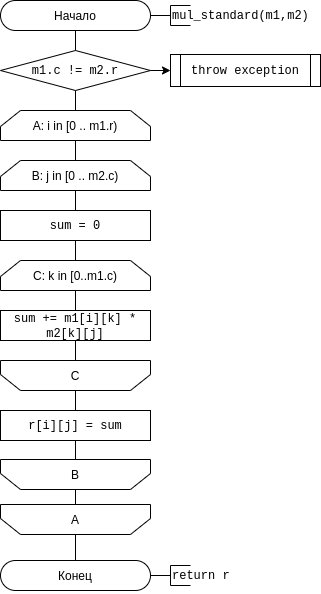
\includegraphics[width=0.7\textwidth]{1/inc/d1.png}
    \caption{Схема рекурсивного алгоритма Левенштейна}
\end{figure}

\pagebreak
\begin{figure}[h]
    \centering
    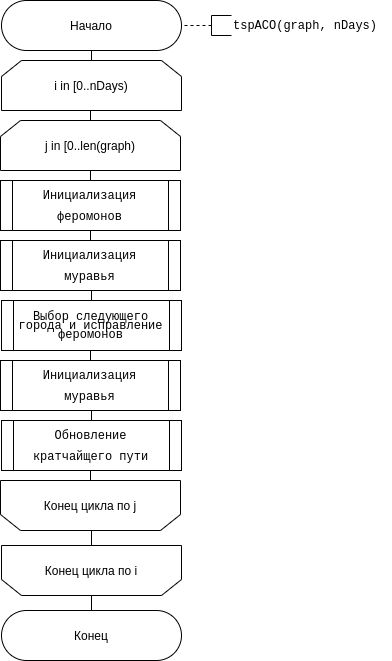
\includegraphics[width=0.65\textwidth]{1/inc/d2.png}
    \caption{Схема матричного алгоритма Левенштейна}
\end{figure}

\pagebreak
\begin{figure}[h]
    \centering
    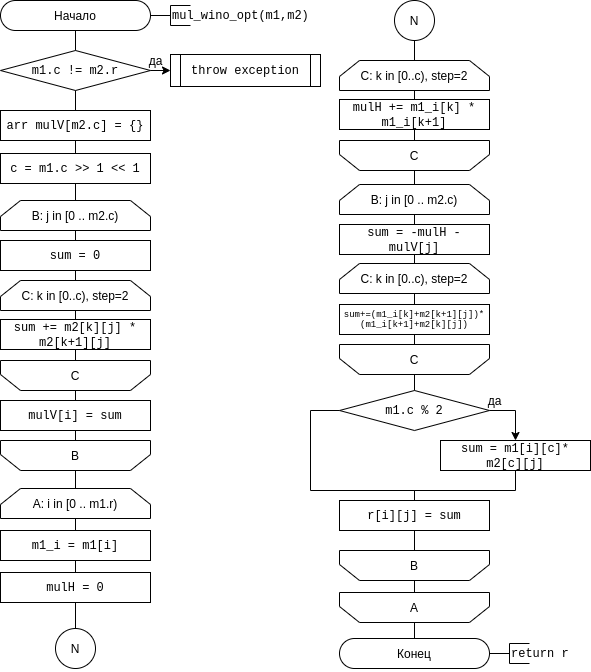
\includegraphics[width=0.8\textwidth]{1/inc/d3.png}
    \caption{Схема мемоизационного алгоритма Левенштейна}
\end{figure}


\newpage
\subsection{Схема алгоритма Дамерау — Левенштейна}

\begin{figure}[]
    \centering
    \includegraphics[width=0.65\textwidth]{1/inc/d4.png}
    \caption{Схема матричного алгоритма Дамерау — Левенштейна}
\end{figure}
\chapter{Технологический раздел}
\label{cha:impl}

В данном разделе будет приведены требования к программу и листинг кода.

\section{Требования к программному обеспечению}

Программа должна принимать в качестве входны данны граф, представленный в виде матрицы смежности.

Результатом программы являются решение задачи коммивояжера для текущего графа.


\section{Средства реализации}

Язык программирования: Go

Редактор: VS Code

Go - это новый мощный язык программирования,
который я учил недавно, поэтому я хочу использовать его на практике.



\section{Листинг кода}

В листингах ниже представлен код программа.

\lstinputlisting[
    language=go,linerange={0-300},tabsize=4,
    caption=Файл main.go
    ]{../src/6/main.go}

\lstinputlisting[
    language=go,linerange={0-300},tabsize=4,
    caption=Файл ant.go
    ]{../src/6/ant.go}

\lstinputlisting[
    language=go,linerange={0-300},tabsize=4,
    caption=Файл utils.go
    ]{../src/6/utils.go}

\section{Вывод}

В этом разделе было рассмотрено требования к программу и кода программы.
\chapter{Экспериментальный раздел}
\label{cha:research}

В данном разделе будет приведено пример работы программы,
результаты тестирования и сравнение времени работы
последовательного и параллельного алгоритма Винограда.

\section{Примеры работы}
На рисунке \ref{fig:4.1} приведен пример работы программы.

\begin{figure}[h]
    \centering
    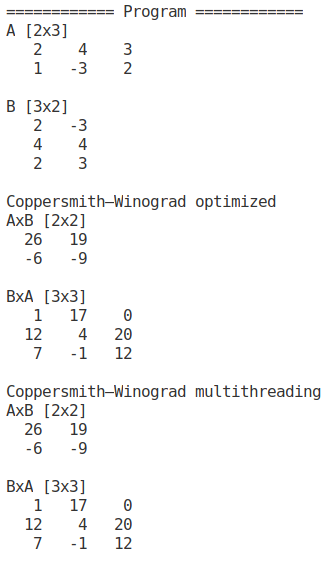
\includegraphics[width=0.4\textwidth]{4/inc/e1.png}
    \caption{Примеры работы программы}
    \label{fig:4.1}
\end{figure}


\section{Результаты тестирования}

На рисунке \ref{fig:4.2} приведен результат теста с использованием фреймворка google test.

\begin{figure}[h]
    \centering
    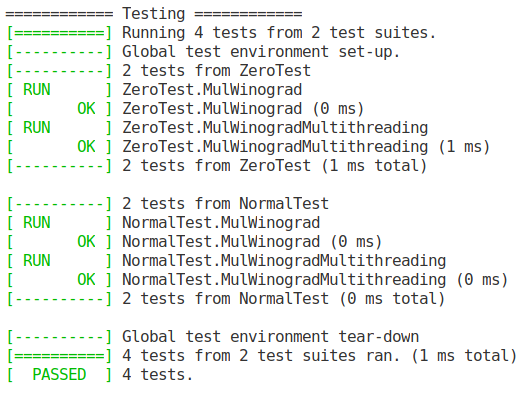
\includegraphics[width=0.6\textwidth]{4/inc/test.png}
    \caption{Результаты тестирования}
    \label{fig:4.2}
\end{figure}


% \section{Постановка эксперимента по замеру времени}
\pagebreak
\section{Сравнение времени работы}

Операционная система - Ubuntu 20.04.1 LTS

Процессор - Intel® CoreTM i5-7300HQ CPU @ 2.50GHz × 4 (ЦП 4 ядра 4 потока)

В таблице \ref{tabular:benchmark} приведены замеры времени
работы алгоритмов умножения матриц на квадратных матрицах,
на основе них построены графики \ref{fig:4.4}.
(На графике 5 графиков.
Графики при использовании 4 потоков и 8 потоков практически идентичны.
Потому что 4 разных потока не усложняют работу ОС.)



% \def\arraystretch{1.2}
\setlength\tabcolsep{0.1cm}

\begin{table}[h]
    \centering
    \csvreader[tabular=|c|c|c|c|c|c|,
        table head=\hline
        \bfseries Размер
        & \bfseries Последо.
        & \bfseries 1 поток
        & \bfseries 2 поток
        & \bfseries 4 поток
        & \bfseries 8 поток
        \\\hline,
        late after line=\\\hline]
        {4/inc/benchmark.csv}{}
    { \csvcoli & \csvcolii & \csvcoliii & \csvcoliv & \csvcolv & \csvcolvi}
    % \csvautotabular{2/inc/benchmark2.csv}
    \caption{\label{tabular:benchmark} Времени работы (ns)}
\end{table}

\begin{figure}[h]
    \centering
    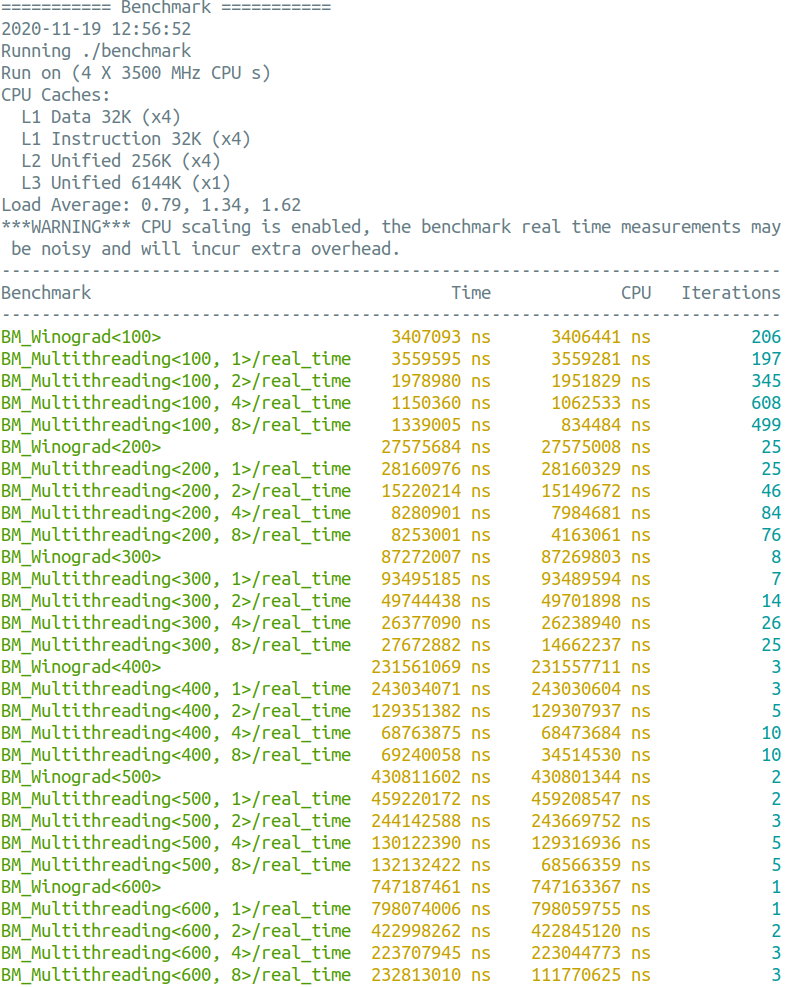
\includegraphics[width=0.9\textwidth]{4/inc/e2.png}
    \caption{Время работы измерено с использованием Google benchmark}
    \label{fig:4.3}
\end{figure}


\clearpage
\begin{figure}[!h]
    \centering
    \begin{tikzpicture}
        \begin{axis}[
            scale=2,
            axis lines=left,
            xlabel=Размер матрицы,
            ylabel={Время, нс},
            legend pos=north west,
            xmajorgrids=true,
            ymajorgrids=true
        ]
            \addplot table[x=n,y=t0,col sep=comma] {4/inc/benchmark.csv};
            \addplot table[x=n,y=t1,col sep=comma] {4/inc/benchmark.csv};
            \addplot table[x=n,y=t2,col sep=comma] {4/inc/benchmark.csv};
            \addplot table[x=n,y=t4,col sep=comma] {4/inc/benchmark.csv};
            \addplot table[x=n,y=t8,col sep=comma] {4/inc/benchmark.csv};
            \legend{Последовательный, 1 поток, 2 поток, 4 поток, 8 поток}
        \end{axis}
    \end{tikzpicture}
    \caption{Зависимость времени работы алгоритмов умножения матриц от размеры матрицы и количество потоков}
    \label{fig:4.4}
\end{figure}


% \section{Сравнительный анализ на материале экспериментальных данных}
% эксперименты+выводы

\section{Вывод}

График показывает, что многопоточная версия более эффективна,
когда количество потоков увеличивается, производительность пропорциональна количеству потоков до тех пор,
пока она не станет равной количеству ядер процессора, и наиболее эффективна,
когда количество потоков равно количеству ядер процессора.
Затем, если количество потоков увеличивается, происходит небольшое уменьшение
из-за необходимости управлять большим количеством потоков.

\chapter*{Заключение}
\addcontentsline{toc}{chapter}{Заключение}

В ходе лабораторной работы было изучено параллельных вычисления
с использованием алгоритма Винограда, реализованны
последовательный и параллельный алгоритм Винограда.
Было сравнить временные характеристики последовательного и параллельного алгоритма Винограда
и сделаны следующие выводы:

\begin{itemize}
    \item производительность пропорциональна количеству потоков до тех пор,
    пока она не станет равной количеству ядер процессора;
    \item многопоточная версия наиболее эффективна когда количество потоков равно количеству ядер процессора;
    \item время выполнения с использованием 4 потоков всего 30\% по сравнению с последовательным выполнением.
\end{itemize}

\addcontentsline{toc}{chapter}{Литература}
\bibliographystyle{ugost2008}


\begin{thebibliography}{8}

    \bibitem{b1}
    Воеводин В. В., Воеводин Вл. В. Параллельные вычисления. — СПб: БХВ-Петербург, 2002. — 608 с.

    \bibitem{b2}
    C++ reference
    \\\url{https://en.cppreference.com/w/cpp/thread/thread}

    \bibitem{b3}
    Google Testing Framework
    \\\url{https://github.com/google/googletest}

    \bibitem{b4}
    Google Benchmark
    \\\url{https://github.com/google/benchmark}

\end{thebibliography}

\end{document}

% http://detexify.kirelabs.org/classify.html


% В данном разделе будет приведено описание схем алгоритмов.
% На рис. 1 представлена схема алгоритма
% определения расстояния Левенштейна в матричной реализации

% В этом разделе анализируются существующие алгоритмы построения трехмерных изображений
% и выбираются наиболее подходящие алгоритмы для решения поставленных задач.

% В данном разделе проектируется новая всячина.

% В данном разделе описано изготовление и требование всячины. Кстати,

% В данном разделе проводятся вычислительные эксперименты.